\documentclass[a4paper]{article}

\usepackage{mathrsfs}
% ============================================
%         General Packages
% ============================================
\usepackage{balance}

\usepackage{kotex}      % for Korean
\usepackage{lipsum}     % for dummy text
\usepackage{array}

\usepackage{cite}   % for citation

\usepackage{amsmath,amsfonts}
\usepackage{amssymb}
\usepackage{soul}
\usepackage{mathrsfs}

\usepackage{hyperref}

    \hypersetup{
        pdftoolbar=false,        	% show Acrobat’s toolbar?
        pdfmenubar=false,        	% show Acrobat’s menu?
        pdffitwindow=false,     	% window fit to page when opened
        pdfstartview={FitH},    	% fits the width of the page to the window
        pdftitle={},    	% title
        pdfauthor={},     	% author
        %     pdfsubject={},   	% subject of the document
        %     pdfcreator={},   	% creator of the document
        %     pdfproducer={}, 	% producer of the document
        %     pdfkeywords={keyword1, key2, key3}, % list of keywords
        %     pdfnewwindow=true,      	% links in new PDF window
        colorlinks=true,       	% false: boxed links; true: colored links
        linkcolor=blue,          	% color of internal links (change box color with linkbordercolor)
        citecolor=blue,       	% color of links to bibliography
        filecolor=blue,      	% color of file links
        urlcolor=blue		% color of external links
    }

\usepackage{algorithm}
\usepackage{algorithmic}

\usepackage{epsfig}
\usepackage[dvipsnames]{xcolor}

% MY PACKAGES ===================================

\usepackage{svg}
\usepackage{subfig}

\usepackage{textcomp}
\usepackage{stfloats}
\usepackage{url}
\usepackage{verbatim}
\usepackage{graphicx}
\usepackage{multirow}
\usepackage{multicol}

\let\proof\relax
\let\endproof\relax
\usepackage{amsthm}
\usepackage{lipsum}
\usepackage{tikz}

% 
\usepackage{titlepic}
\usepackage{pdfpages}
\usepackage{etoolbox} % 조건문을 쓰기 위한 패키지


\titlepic{%
  
\includegraphics[height = 8mm]{figures/logo_KAIST_simple.png}
  \hspace{5mm}
  
\includegraphics[height = 8mm]{figures/MIC_Logo.png}
  }

% ========================================
%         TITLE and AUTHORS
% ========================================
\title{
  Online Multistep Lookahead
}

\author{
    Changeun Park
    \thanks{\href{https://kaist-mic-lab.github.io/members/cePark/}{Changeun Park} is an integrated M.S./Ph.D. student at KAIST, {\tt\small aegis3141@kaist.ac.kr}}%
}

\date{
    % 20\textsuperscript{th} March 2025
    Complied on \today
}

\begin{document}

\maketitle

% ========================================
%         Contents
% ========================================

\begin{figure}[h]
  \centering
  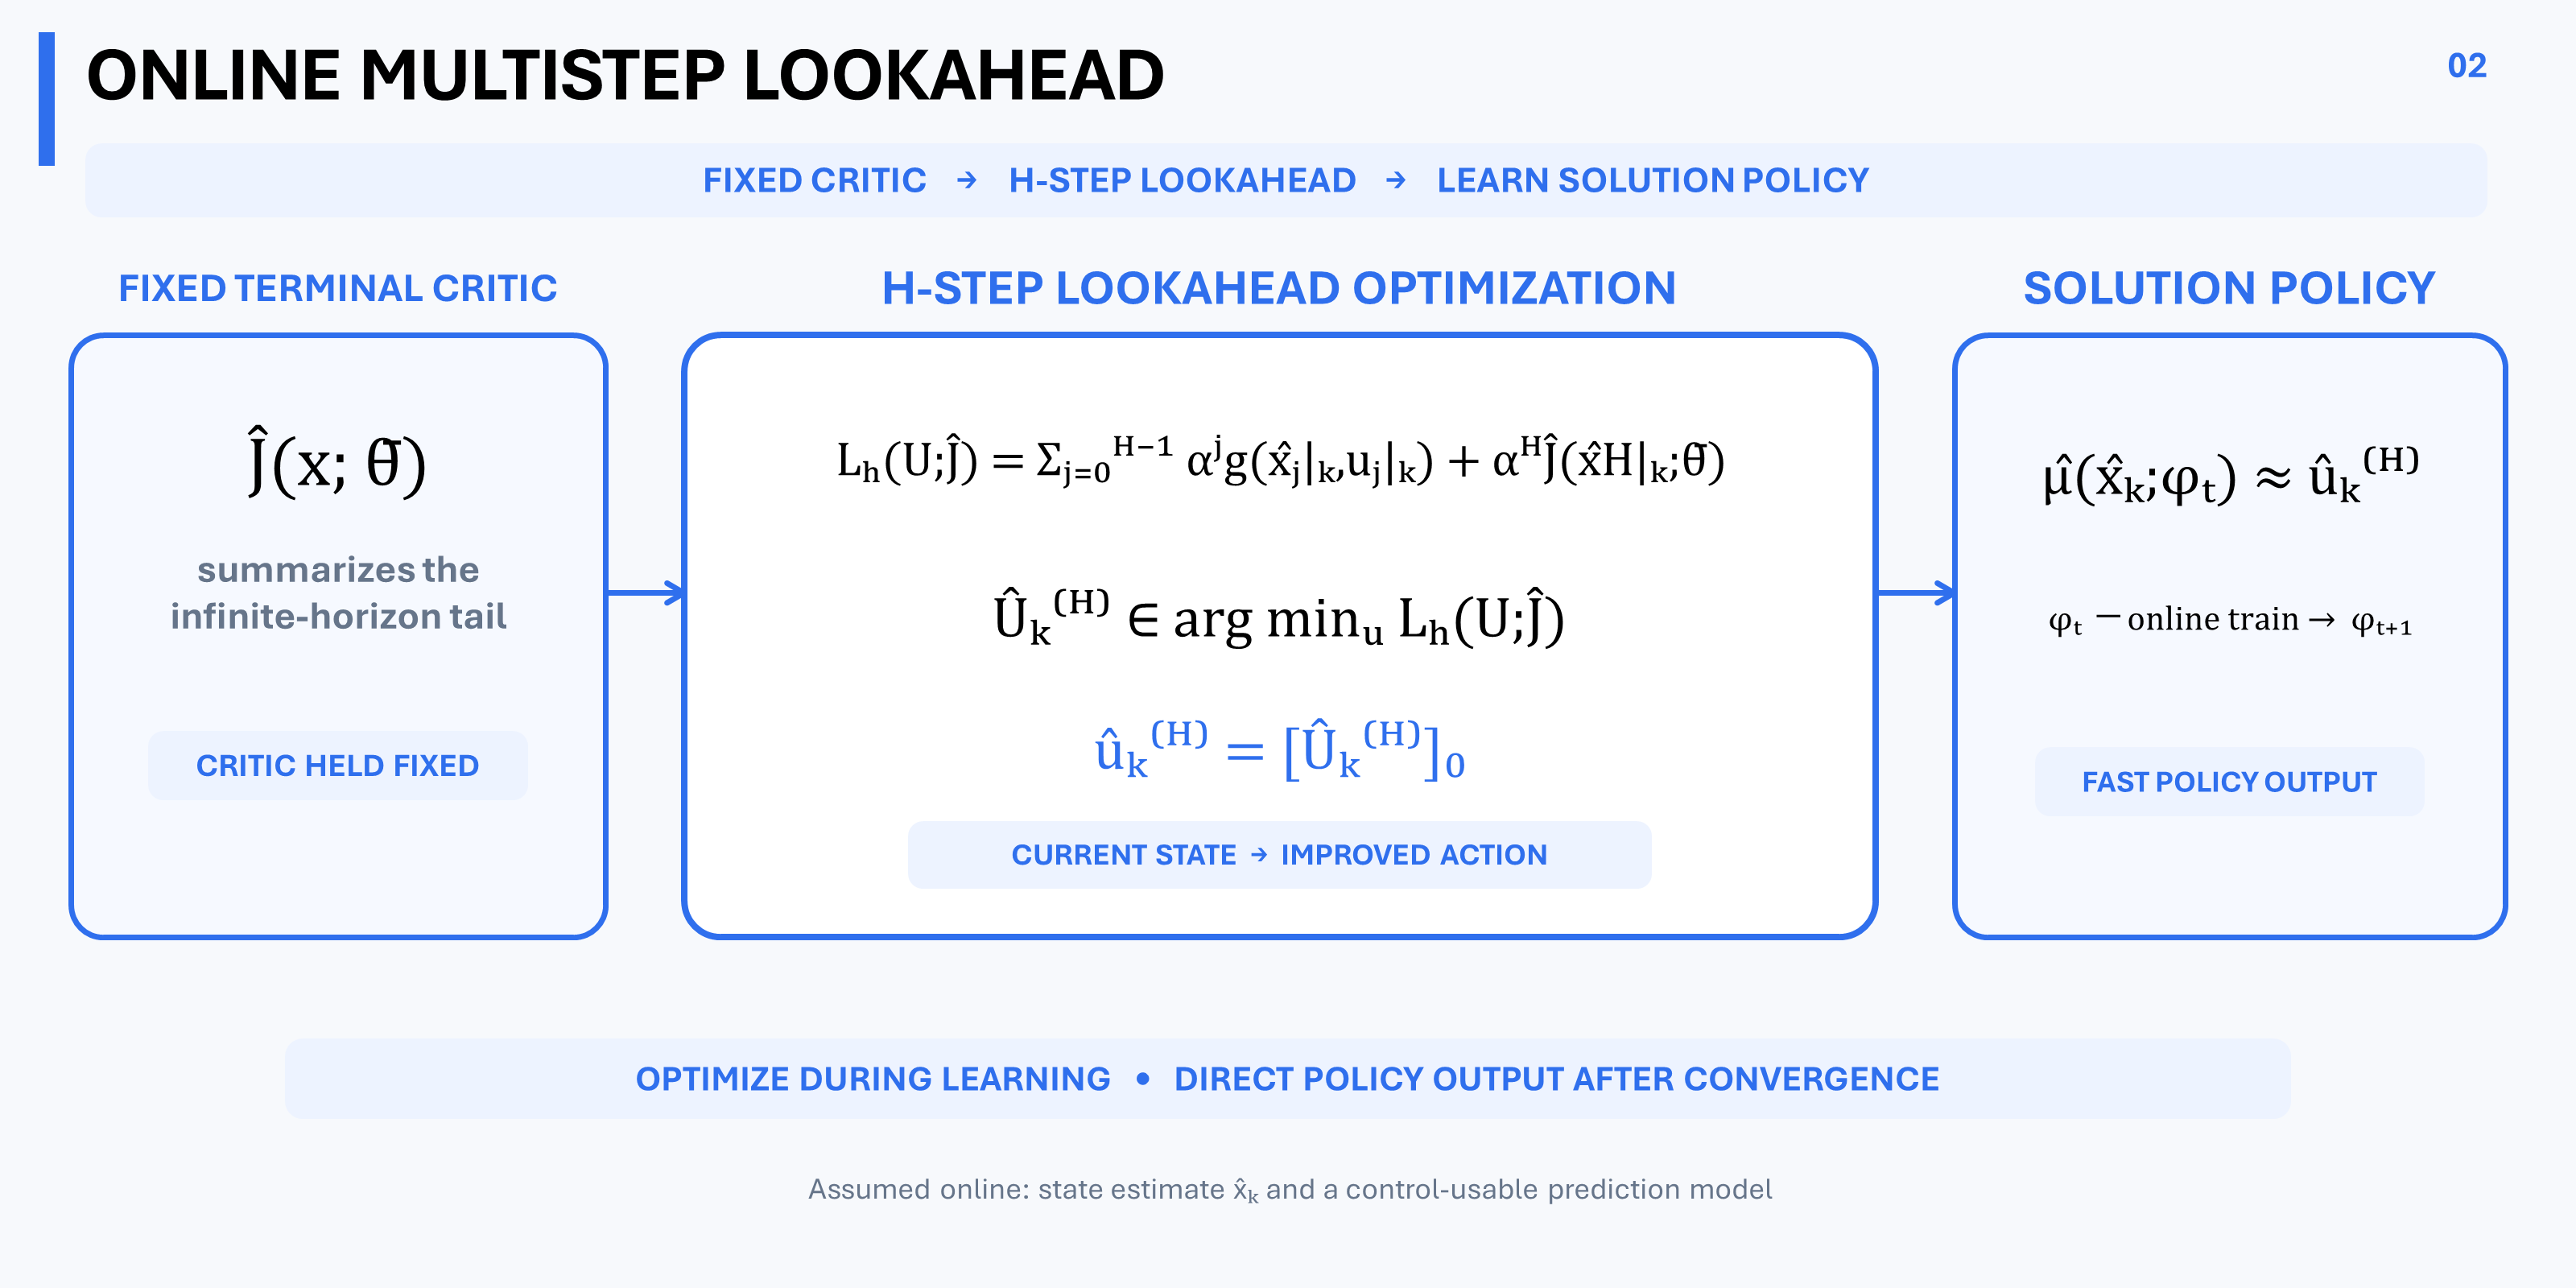
\includegraphics[width=\textwidth]{figures/02_online_multistep_lookahead.png}
\end{figure}

\nocite{*} % <------------ 인용있으면 삭제

Physical interaction is indexed by $k$, whereas policy-network updates are
indexed by $t$. Here $t(k)$ is the latest policy-network update available at
physical step $k$, and $k(t)$ is the latest physical sample available at
learner update $t$. The critic parameter $\bar\theta$ is deliberately fixed
in this Theme. A state estimate $\widehat x_k$ and a control-usable prediction
model $f_{\mathrm{use}}$ are assumed available.

\section{Problem definition}

\href{https://kaist-mic-lab.github.io/research/research_themes/00_online_learning_based_optimal_control/}{Online Learning-Based Optimal Control}
connects an approximate critic to policy improvement through Bellman
minimization. Here the critic is already available but imperfect. Rather than
using only a one-step greedy action, solve an $H$-step problem whose terminal
cost is the fixed critic:

\begin{equation}
  \begin{aligned}
    \widehat U_k^{(H)}
    \in\arg\min_{U_k}\quad&
    \sum_{j=0}^{H-1}
    \alpha^j g(\widehat x_{j|k},u_{j|k})
    +
    \alpha^H\widehat J_{\bar\theta}(\widehat x_{H|k})\\
    \mathrm{s.t.}\quad&
    \widehat x_{0|k}=\widehat x_k,\\
    &
    \widehat x_{j+1|k}
    =
    f_{\mathrm{use}}(\widehat x_{j|k},u_{j|k}),
    \qquad j=0,\ldots,H-1,\\
    &
    u_{j|k}\in\mathcal U(\widehat x_{j|k}),
    \qquad j=0,\ldots,H-1,\\
    &
    \widehat x_{j|k}\in\mathcal X,
    \qquad j=0,\ldots,H,
  \end{aligned}
\end{equation}

\begin{equation}
  \widehat u_k^{(H)}
  =
  \left[\widehat U_k^{(H)}\right]_0 .
\end{equation}

$H$ is a positive lookahead horizon, $0<\alpha<1$ is the discount factor, and
$U_k=(u_{0|k},\ldots,u_{H-1|k})$ is the candidate input sequence.
$f_{\mathrm{use}}$ is the declared prediction model,
$\mathcal U(x)$ and $\mathcal X$ are the admissible input and state sets, and
$\widehat x_{j|k}$ is the state predicted $j$ steps from the current estimate.
$\widehat u_k^{(H)}$ selects the first optimized action. For $H=1$, the
formulation reduces to one-step critic-based policy improvement.

The online-learned policy represents the solution map:

\begin{equation}
  \widehat\mu_{\phi_t}(\widehat x_k)
  \approx
  \widehat u_k^{(H)},
  \qquad
  u_k^{\mathrm{NN}}
  =
  \widehat\mu_{\phi_{t(k)}}(\widehat x_k).
\end{equation}

The critic is not updated in this Theme. The learned object is the policy
induced by the fixed critic and multistep optimization. The model can be known
or a declared snapshot of a learned model, but it is held fixed while each
lookahead problem is solved. Changes in that snapshot, preview convention, or
constraint set between solves move the teacher solution map and must be
represented in the training data or policy input.

\section{Why this problem matters}

An approximate critic summarizes the infinite-horizon tail, but local critic
error can lead to a poor one-step greedy action. Multistep lookahead evaluates
the current action through $H$ explicit stages before applying the critic.
Under suitable discounted-DP and rollout assumptions, this can improve the
policy even while the critic remains fixed, and a longer horizon can reduce
the influence of terminal-critic error. Improvement is possible rather than
automatic: model error, incomplete optimization, and policy approximation can
offset the benefit.

Repeatedly solving the $H$-step problem may still be too expensive for an
embedded controller. Learning its state-to-solution map amortizes the
computation across operating points: lookahead supplies improved action
targets during learning, whereas the converged policy network can return an
action immediately without a full optimization at every control step.

\section{Key challenges}

\begin{itemize}
  \item \textbf{Horizon and model trade-off:} increasing $H$ can reduce dependence on the
  terminal critic but raises computation and accumulated model error.
  \item \textbf{Constrained real-time optimization:} nonlinear dynamics and constraints
  create feasibility, local-solution, warm-start, and worst-case latency
  issues.
  \item \textbf{Solution-policy learning:} targets are concentrated on visited states,
  and a small action-fitting error does not by itself imply small closed-loop
  performance loss.
  \item \textbf{Safe deployment:} approximating a feasible optimizer does not
  automatically preserve feasibility or stability; a correction solve,
  projection, safety filter, or fallback may remain necessary.
\end{itemize}

\section{A conventional approach — repeated online lookahead}

A conventional realization solves the problem in Section 1 at every physical
control step and applies only the first action:

\begin{equation}
  u_k=\widehat u_k^{(H)},
  \qquad
  k=0,1,\ldots .
\end{equation}

This receding-horizon implementation uses the current state, model, critic,
and constraints directly. Its main limitation is repeated numerical
optimization within the control deadline.

This mechanism is MPC-like, but its defining role here is more specific: the
fixed approximate infinite-horizon critic closes the finite lookahead problem.
Learning a conventional finite-horizon MPC solution without that terminal
critic remains a useful amortized-MPC baseline, not this Theme's defining
mechanism.

\section{Research direction — online learning of the lookahead solution}

Let selected online lookahead targets be

\begin{equation}
  \mathcal S_t^{\mathrm{LA}}
  \subseteq
  \left\{
  \left(\widehat x_i,\widehat u_i^{(H)}\right)
  \right\}_{i=0}^{k(t)} .
\end{equation}

A conceptual policy-learning problem is

\begin{equation}
  \phi_{t+1}
  \approx
  \arg\min_{\phi}
  \sum_{(x,u^{(H)})\in\mathcal S_t^{\mathrm{LA}}}
  \left\|
  \widehat\mu_{\phi}(x)-u^{(H)}
  \right\|_{W_u}^{2}.
\end{equation}

Here $W_u\succeq 0$ is the declared action-fitting weight matrix.

Equivalently, the research loop can be summarized as

\begin{equation}
  \widehat J_{\bar\theta}\ \text{fixed},
  \qquad
  \phi_t
  \xrightarrow[\mathcal S_t^{\mathrm{LA}}]
  {\text{online solution learning}}
  \phi_{t+1},
  \qquad
  u_k^{\mathrm{NN}}
  =\widehat\mu_{\phi_{t(k)}}(\widehat x_k).
\end{equation}

The argmin states the learning objective; a real-time implementation may take
only one or a few incremental updates. Training signals may come from a
completed lookahead solve or a corrected warm start. If necessary, deployment
can retain a real feasibility mechanism,

\begin{equation}
  u_k
  =
  \mathcal C_{\mathrm{feas}}
  \left(
  \widehat\mu_{\phi_{t(k)}}(\widehat x_k),
  \widehat x_k
  \right),
\end{equation}

where $\mathcal C_{\mathrm{feas}}$ must denote an implemented projection,
filter, or correction procedure rather than an assumed guarantee.

Evidence should compare the network action and objective with the online
optimizer, constraint violations before and after correction, closed-loop
cost, worst-case latency, model and critic perturbations, and performance on
states not represented in the update stream. This page states the research
direction and evaluation criteria; it does not claim a validated MIC Lab
result.

\section{Application domains}

\begin{itemize}
  \item \textbf{Electric-drive current or torque control:} combine a learned terminal
  critic with short online lookahead to make an approximate infinite-horizon
  MPC realization practical.
  \item \textbf{Coordination of multiple connected and automated vehicles and other
  complex decision problems:} use multistep optimization to generate a
  high-quality policy target, amortize that target into a fast policy network,
  or use the lookahead action as an online policy-improvement target within an
  RL framework.
  \item \textbf{Vehicle energy and thermal management:} represent long-horizon
  consequences with the terminal critic while multistep lookahead resolves
  short-horizon dynamics, constraints, and current operating information.
  \item \textbf{Embedded motion control and MPC-like systems} where a reliable optimizer
  is available during learning but too costly for permanent execution.
\end{itemize}

\section{References}

\begin{itemize}
  \item D. P. Bertsekas, \textit{Reinforcement Learning and Optimal Control}, Athena
  Scientific, 2019.
  \item D. P. Bertsekas, \textit{A Course in Reinforcement Learning}, 2nd ed., Athena
  Scientific, 2025.
\end{itemize}

% ========================================
%         Appendix
% ========================================

% \begin{appendices}
% \end{appendices}

\addcontentsline{toc}{chapter}{Bibliography}
\bibliographystyle{IEEEtran}
\bibliography{refs}

\end{document}
